% Author: Rasmus Pank Roulund
% Inspired by figure in:
% Howells, Peter og Bain, Keith (2007). Financial markets and
% institutions. 5. udg. Essex: Pearson Education.
\documentclass{standalone}
\usepackage{tikz}
\usepackage{verbatim}

\usetikzlibrary{arrows,positioning} 
\tikzset{
    %Define standard arrow tip
    >=stealth',
    %Define style for boxes
    punkt/.style={
           rectangle,
           rounded corners,
           draw=black, very thick,
           text width=6.5em,
           minimum height=2em,
           text centered},
    % Define arrow style
    pil/.style={
           ->,
           thick,
           shorten <=2pt,
           shorten >=2pt,}
}

\begin{document}

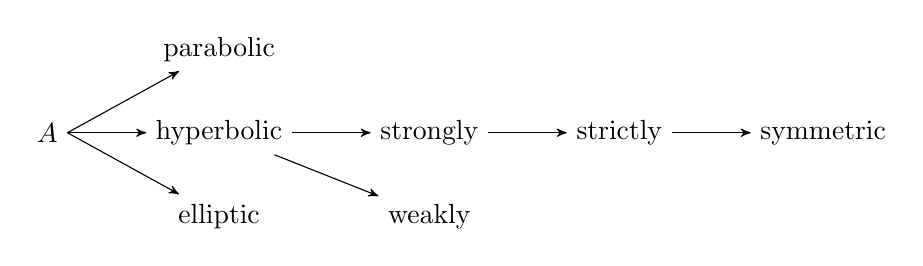
\begin{tikzpicture}[node distance=1cm]
 \node (A) {$A$};
 \node[right=of A] (hyperbolic) {hyperbolic}
     edge[<-] (A.east); 
 \node[above=0.5cm of hyperbolic] (parabolic) {parabolic}
     edge[<-] (A.east); 
 \node[below=0.5cm of hyperbolic] (elliptic) {elliptic}
     edge[<-] (A.east);
     
 \node[right=of hyperbolic] (strongly) {strongly}
     edge[<-] (hyperbolic);
 \node[below=0.5cm of strongly] (weakly) {weakly}
     edge[<-] (hyperbolic);
     
 \node[right=1cm of strongly] (strictly) {strictly}
     edge[<-] (strongly);
     
 \node[right=of strictly] (symmetric) {symmetric}
     edge[<-] (strictly);
\end{tikzpicture}
\end{document}